
% Modelo de Trabalho Acadêmico da UNESP de Guaratinguetá v-2.1
% atualização Copyright 2024 by Biblioteca FEG UNESP com colaboração de Vitor Pinto Ribeiro and Gustavo Santos Borges and Ronaldo César de Paiva
% Modelo de Trabalho Acadêmico da UNESP de Guaratinguetá v-1.0
% original copyright 2017 by Eduardo Rohde Eras

% This program is free software: you can redistribute it and/or modify
% it under the terms of the GNU General Public License as published by
% the Free Software Foundation, either version 3 of the License, or
% (at your option) any later version.
%
% This program is distributed in the hope that it will be useful,
% but WITHOUT ANY WARRANTY; without even the implied warranty of
% MERCHANTABILITY or FITNESS FOR A PARTICULAR PURPOSE.  See the
% GNU General Public License for more details.
%
% You should have received a copy of the GNU General Public License
% along with this program.  If not, see <http://www.gnu.org/licenses/>.
%
%----------------------------------------------------------------------------------------%
%APRESENTAÇÃO 
% Este modelo pode ser usado como apoio para seu trabalho acadêmico e é destinado para ser usado no Word, não aplicável a outros editores de texto.
%
%Essas instruções são voltadas para a comunidade acadêmica da Universidade Estadual Paulista “Júlio de Mesquita Filho” (Unesp). Caso você seja de outra instituição, verifique as regras vigentes da sua universidade ou faculdade.
%
%O uso deste modelo não substitui o conhecimento das normas, diretrizes da universidade e orientações de seus professores e a Rede de Bibliotecas da Unesp está isenta de eventuais e quaisquer problemas ou prejuízos decorrentes do uso deste arquivo em softwares não licenciados, arquivos corrompidos, vírus ou quaisquer outros motivos.
%
%Em caso de dúvidas, consulte o Manual de normalização de trabalhos acadêmicos: apresentação: ABNT (2023): \url{https://docs.google.com/document/d/1ipkGiAUnAr_YBTrpFJpnud3aa4llBsROpBdkUfw91L0/edit?usp=sharing}
%----------------------------------------------------------------------------------------%
% C L A S S E   D O   D O C U M E N T O
%----------------------------------------------------------------------------------------%

\PassOptionsToPackage{colorlinks=true, allcolors=black}{hyperref}
\documentclass[
  %----------------------------------------------------------------------------------------%
  %Opções da classe 'memoir'
  %----------------------------------------------------------------------------------------%
  12pt,		% Tamanho da Fonte.
  a4paper,	% Tamanho da página.
  openright,  % Capítulos começam em páginas ímpares (insere uma página vazia se necessário).
  oneside,	% Para impressão em frente e verso utilizar twoside.
  %----------------------------------------------------------------------------------------%
  %Opções da classe 'abntex2'
  %----------------------------------------------------------------------------------------%
  chapter=TITLE,		%Títulos de capítulos convertidos em letras maiúsculas.
  section=TITLE,		%Títulos de seções convertidos em letras maiúsculas.
  %----------------------------------------------------------------------------------------%
  %Opções da classe 'babel'
  %----------------------------------------------------------------------------------------%
  english,	%Idioma adicional para hifenização.
  french,	    %Idioma adicional para hifenização.
  spanish,	%Idioma adicional para hifenização.
  brazil	    %Idioma principal do documento.
  %----------------------------------------------------------------------------------------%
]{abntex2}

%----------------------------------------------------------------------------------------%
% P A C O T E S
%
% Insira aqui os pacotes que for utilizar em seu documento. Para saber quais pacotes o
% template já está utilizando, confira o arquivo "pacoteBasico.sty".
%----------------------------------------------------------------------------------------%
    
    \usepackage{pacoteBasico}   %Pacote Básico de formatação no padrão da UNESP/FEG
    \usepackage{color}		    %Controle das cores.
    \usepackage{graphicx}	    %Inclusão de gráficos.
    \usepackage{lipsum}		    %Para geração de 'Dummy Text'.
    \usepackage{pdfpages}       %Para inclusão de arquivos pdf
    \usepackage[table,xcdraw]{xcolor}


	% Para gerar Fluxograma
	\usepackage{tikz}
	\usetikzlibrary{shapes.geometric, arrows.meta, positioning}
	\tikzstyle{caixa} = [rectangle, rounded corners, minimum width=4cm, minimum height=1cm,text centered, draw=black, fill=gray!10]
	\tikzstyle{seta} = [thick,->,>=stealth]




\begin{document}
    
%----------------------------------------------------------------------------------------%
% I N F O R M A Ç Õ E S   B Á S I C A S   S O B R E   O   T R A B A L H O
%
% Defina aqui as informações pertinentes ao trabalho.
%----------------------------------------------------------------------------------------%

%----------------------------------------------------------------------------------------%
% D A D O S   P E S S O A I S
%----------------------------------------------------------------------------------------%

%Nome completo do autor do presente Trabalho acadêmico:
\newcommand{\nomeDoAutor}{
	Jonas Ernesto Poli
}

%Nome do curso:
\newcommand{\nomeDoCurso}{Programa de Pós Graduação em Ciência, Tecnologia e Sociedade}

%----------------------------------------------------------------------------------------%
% D A D O S   S O B R E   O   T R A B A L H O
%----------------------------------------------------------------------------------------%

%Título do presente trabalho:
\newcommand{\tituloDoTrabalho}{
	Título do trabalho acadêmico
}

%Subtítulo do presente trabalho, se houver:
\newcommand{\subtituloDoTrabalho}{
	subtítulo se houver
}

%Tipo do trabalho (Dissertação / Tese / Trabalho de Conclusão de Curso / Trabalho de Conclusão de Residencia) 
\newcommand{\tipoDeTrabalho}{Tipo de Trabalho Acadêmico}

% Nome da Faculdade ou instituto
\newcommand{\NomeDaFaculdade}{UFSCAR}

%Grau acadêmico (Mestre(a) / Doutor(a) / Bachareal / Licenciatura etc)
\newcommand{\GrauAcademico}{Mestre}

% área de concentração, se houver (muito utilizado no mestrado e doutorado) % remover no pacote básico se não houver 
\newcommand{\AreaDeConcentracao}{
	Área de concentração
}

%Mês da entrega do trabalho 
\newcommand{\dataDeDefesa}{
	99/99/9999
}

%Ano da entrega do trabalho
\newcommand{\anoDeEntrega}{
	2025
}

%----------------------------------------------------------------------------------------%
% D A D O S   D O S   O R I E N T A D O R E S,   B A N C A   E   C O O R D E N A D O R
%----------------------------------------------------------------------------------------%

%Nome do orientador do presente trabalho:
\newcommand{\nomeDoOrientador}{
	Nome Completo do Orientador
}
% acrescentar intituição 
%Título do orientador:
\newcommand{\tituloDoOrientador}{
	Profº Dr.
}

%Nome do coorientador, se houver:
\newcommand{\NomeDoCoorientador}{
	Nome Completo do Coorientador
}

%Título do coorientador:
\newcommand{\tituloDoCoorientador}{
	Profº Dr.
}

%instituição do orientador 
\newcommand{\instituicaoorientador}{Nome da Instituição do orientador}     

%instituição do coorientador 
\newcommand{\instituicaocoorientador}{Nome da Instituição do coorientador}

%Nome do Membro da Banca 1 :
\newcommand{\nomeDoMembroA}{Nome Completo do Membro da Banca}

%Título do Membro da Banca 1:
\newcommand{\tituloDoMembroA}{Profº Dr.}
%instituição do Membro da Banca 1 
\newcommand{\instituicaomembroA}{Nome da Instituição do membro 1}

%Nome do membro da Banca 2:
\newcommand{\nomeDoMembroB}{Nome Completo do Membro banca}

%Título do Membro da Banca 2:
\newcommand{\tituloDoMembroB}{Profº Dr.}
% Instituição do Membro 2
\newcommand{\instituicaomembroB}{Nome da Instituição do membro 2}

%ATENÇÃO! Geralmente Tese de Doutorado possui mais de 2 membros na banca, então é possível remover no pacote básico. 
%Nome do membro da Banca 3:
\newcommand{\nomeDoMembroC}{Nome Completo do Membro banca}

%Título do Membro da Banca 3:
\newcommand{\tituloDoMembroC}{Profº Dr.}
% Instituição do Membro 3
\newcommand{\instituicaomembroC}{Nome da Instituição do membro 3}
%Nome do membro da Banca 4:
\newcommand{\nomeDoMembroD}{Nome Completo do Membro banca}

%Título do Membro da Banca 4:
\newcommand{\tituloDoMembroD}{Profº Dr.}
% Instituição do Membro 4
\newcommand{\instituicaomembroD}{Nome da Instituição do membro 4}
%----------------------------------------------------------------------------------------%
% D A D O S   D A   I N S T I T U I Ç Ã O
%----------------------------------------------------------------------------------------%

%Nome da Cidade de defesa
\newcommand{\nomeDaCidade}{São Carlos}

%Nome da Universidade Nome da Faculdade ou Instituto - Campus nome da Cidade

\newcommand{\nomeDaUniversidade}{
	Universidade Federal de São Carlos - UFSCAR\\
	\NomeDaFaculdade -- Campus de\ \nomeDaCidade
}




%----------------------------------------------------------------------------------------%
% I N Í C I O   D O   D O C U M E N T O - P R É   T E X T U A L

%----------------------------------------------------------------------------------------%






\begin{center}
	\setstretch{1.75}
	\textbf{\LARGE AgroSíntese:}\\[0.5em]
	\textbf{\LARGE Uma Plataforma Dialógica e Inclusiva de ATER via WhatsApp com Inteligência Artificial e Regionalismos Linguísticos}\\[0.5em]
\end{center}

\vspace{2em}

\begin{center}
	\setstretch{1}
	\textbf{Jonas Ernesto Poli}\\
	Mestrando em Ciência, Tecnologia e Sociedade pela Universidade\\
	Federal de São Carlos, Brasil.\\
	E-mail: \href{mailto:jonaspoli@ufscar.br}{jonaspoli@ufscar.br}
\end{center}

\vspace{2em}

\begin{center}
	\setstretch{1}
	\textbf{Luís Fernando Soares Zuin}\\
    Doutor em Engenharia de Produção\\
	Federal de São Carlos, Brasil. Professora da Universidade Federal de\\
	São Carlos, Brasil.\\
	E-mail: \href{mailto:zuin@ufscar.br}{zuin@ufscar.br}
\end{center}
	
	
	%------------------------------------------------------------------------------------%
	% R E S U M O   N O   I D I O M A   D O   T E X T O
	%
	% OBRIGATÓRIO. Elaborado conforme a NBR 6028. 
	% Deve ser redigido em um só parágrafo contendo de 150 a 500 palavras e ressaltar: objetivo, método, resultados e as principais conclusões.
	% Após o resumo, são listadas palavras-chave relacionadas à temática do trabalho, separadas entre si por ponto e virgula (;) e finalizadas por ponto final.  (NBR 6028)
	%------------------------------------------------------------------------------------%
	
	\begin{resumo}
		\setstretch{1}
		Este artigo apresenta o AgroSíntese, um sistema inovador de Assistência Técnica e Extensão Rural (ATER), baseado em inteligência artificial (IA) e integrado ao WhatsApp, que busca atender às necessidades específicas dos agricultores familiares brasileiros por meio de uma comunicação dialógica e culturalmente situada. O AgroSíntese utiliza o modelo de IA GPT4All, treinado com conteúdos técnicos agrícolas específicos e regionalizados, permitindo que as respostas geradas sejam personalizadas em texto ou áudio, com síntese de voz adaptada aos sotaques e expressões regionais brasileiras. A fundamentação teórica deste trabalho baseia-se principalmente nas contribuições de Mikhail Bakhtin sobre o dialogismo e o caráter social da linguagem, na abordagem educativa crítica e dialógica de Paulo Freire, na visão da experiência como elemento transformador proposta por Jorge Larrosa e nas perspectivas sobre comunicação rural e digitalização da extensão rural desenvolvidas por Luís Fernando Soares Zuin e Renato Lopes. O AgroSíntese visa democratizar e facilitar o acesso ao conhecimento técnico agrícola, aumentando significativamente a inclusão digital, a compreensão e aplicação prática das técnicas agrícolas pelos agricultores. Além disso, espera-se promover o fortalecimento das identidades culturais locais e da autonomia produtiva e social das comunidades rurais, alinhando-se aos Objetivos de Desenvolvimento Sustentável (ODS) da ONU. Em termos práticos, a utilização dessa tecnologia prevê impactos positivos diretos na produtividade agrícola, na sustentabilidade econômica e na valorização das diversidades linguísticas e culturais do Brasil rural.
		
		\vspace*{0.5cm}
		
		\noindent\textbf{{Palavras-Chave: }} Assistência Técnica e Extensão Rural; Inteligência Artificial; GPT4All; Comunicação Dialógica; Agricultura Familiar; WhatsApp; ATER Digital Participativa.
		
	\end{resumo}
	
	%------------------------------------------------------------------------------------%
	% A B S T R A C T :   R E S U M O   N O   I D I O M A   E S T R A N G E I R O
	%
	% OBRIGATÓRIO. Elaborado com as mesmas características do resumo em língua portuguesa.
	% Se redigido em inglês-ABSTRACT, em castelhano-RESUMEN, em francês-RÉSUMÉ.
	% Após o resumo, são listadas palavras-chave relacionadas à temática do trabalho no 
	% idioma escolhido. Se redigido em inglês - KEYWORDS, em espanhol - PALABRAS CLAVES,
	% em francês - MOTS-CLÉS.
	% TEXTO ATUAL 
	%ZUSAMMENFASSUNG (alemão)
	%RIASSUNTO (italiano)
	
	%Keywords (inglês)
	%Palabras clave (espanhol)
	%Mot-clé (francês)
	%Stichwörter (alemão)
	%Parole chiave (italiano)
	%------------------------------------------------------------------------------------%
	\begin{center}
		\setstretch{1}
		\textbf{\large AgroSynthesis: A Dialogical and Inclusive ATER Platform via WhatsApp with Artificial Intelligence and Linguistic Regionalisms}
	\end{center}	
	\begin{resumo}[Abstract] % Substitua 'Abstract' pela palavra no idioma desejado, caso precise.
		\setstretch{1}
		This paper presents AgroSíntese, an innovative Technical Assistance and Rural Extension (ATER) system based on artificial intelligence (AI) integrated with WhatsApp, designed specifically to address the unique communication and technical needs of Brazilian family farmers. AgroSíntese employs the GPT4All AI model, specially trained with regionally adapted agricultural content, enabling personalized textual and audio responses through speech synthesis technology attuned to the regional accents and linguistic nuances of Brazil. The theoretical foundation of this study draws primarily from Mikhail Bakhtin's concepts of dialogism and the inherently social nature of language, Paulo Freire's critical and dialogical educational approach, Jorge Larrosa’s emphasis on experience as transformative, and Luís Fernando Soares Zuin and Renato Lopes’ work on rural communication and digital extension methodologies. AgroSíntese seeks to democratize access to specialized agricultural knowledge, significantly enhancing digital inclusion and ensuring clearer understanding and practical implementation of farming techniques. Furthermore, it aims to strengthen local cultural identities and the productive and social autonomy of rural communities, contributing to the United Nations' Sustainable Development Goals (SDGs). Practically, the deployment of this technology is expected to yield direct positive impacts on agricultural productivity, economic sustainability, and the recognition and preservation of Brazil’s diverse linguistic and cultural landscapes in rural settings.
		
		\vspace*{0.5cm}
		
		%Subistitua 'Keywords' pela palavra no idioma desejado, caso precise.
		\noindent\textbf{{Keywords: }} Technical Assistance and Rural Extension; Artificial Intelligence; GPT4All; Dialogical Communication; Family Farming; WhatsApp; Participatory Digital Extension.
		
		
	\end{resumo}
	

	
	

	


    \newpage
    
    %------------------------------------------------------------------------------------%
    %                                                                                    %
    %                           C O R P O   D O   T E X T O                              %
    %                                                                                    %
    %                     Seu trabalho começa a ser digitado aqui.                       %
    %                                                                                    %
    % Início do corpo do texto. A partir desse comando será impresso o número de páginas.% 
    %------------------------------------------------------------------------------------%
    
    \textual
    \pagestyle{simple} 
    
    %------------------------------------------------------------------------------------%
    
     \chapter{Introdução} % ELEMENTO OBRIGATÓRIO

\begin{flushleft}


A notável diversidade linguística que caracteriza as múltiplas regiões do Brasil configura-se como uma das mais ricas expressões da complexidade cultural da nação. Pode-se afirmar, sem exagero, que essa pluralidade, disseminada por todo o território, encerra uma memória histórica que resistiu ao tempo, preservada fundamentalmente na oralidade do cotidiano. Esta riqueza manifesta-se não apenas através dos distintos sotaques regionais, mas também pela presença de idiomas completos, como os falados por comunidades indígenas mais isoladas e por descendentes de imigrantes.

Diante dessa complexidade, inúmeros trabalhos buscaram identificar e sistematizar os idiomas e variantes falados no Brasil. Destacam-se desde estudos pioneiros, como os de Antenor \cite{nascentes1953}, iniciados em 1922, que propuseram uma organização da fala brasileira em zonas dialetais, até investigações mais recentes e abrangentes, como as conduzidas pelo projeto Atlas Linguístico do Brasil (ALiB). Este último dedica-se à análise e organização das variadas formas de expressão do português e de outras línguas presentes no país \cite{cardoso2014alib, Aguilera2022}.

Contudo, um desafio persistente apontado por diversos estudos é a progressiva diminuição das diferenças linguísticas. As formas de falar do brasileiro, por vezes incentivadas ou mesmo forçadas por dinâmicas sociais e culturais, tendem a uma crescente homogeneização. Para dimensionar a questão dos sotaques, é importante analisar um fenômeno parecido que afeta os idiomas no Brasil. Gilvan Müller de Oliveira identificou que, atualmente, são falados cerca de 210 idiomas no país. As populações indígenas utilizam aproximadamente 170 dessas línguas (conhecidas como autóctones), enquanto comunidades de descendentes de imigrantes mantêm vivas em torno de 30 línguas (denominadas alóctones). Adicionalmente, existem duas línguas de sinais empregadas pelas comunidades surdas: a Língua Brasileira de Sinais (Libras) e a língua de sinais Urubu-Kaapór. Estes números confirmam o Brasil como um país multilíngue, como acontece com a maioria das nações globais \cite{noauthor_plurilinguismo_nodate}.

Apesar dessa riqueza, os dados históricos indicam uma perda significativa dessa diversidade. Conforme apontado por \cite{rodrigues_linguas_nodate}, há pouco mais de cinco séculos, existiam aproximadamente 1.078 línguas distintas em uso. Hoje, mesmo com um expressivo aumento populacional, o número de idiomas falados reduziu-se drasticamente. Essa constatação evidencia a urgência na criação de mecanismos para a preservação da diversidade linguística que ainda existe. Além do valor cultural da própria preservação da forma de falar; ainda torna necessário diante dos riscos de exclusão digital por parte de alguns e da perpetuação de vieses linguísticos em tecnologias emergentes, como a inteligência artificial. A ausência de tecnologias linguisticamente conscientes pode agravar desigualdades, dificultando o acesso à informação e a serviços por parte de falantes de uma variedades linguística "não padrão".

Este cenário levanta uma questão fundamental de natureza política e cultural: como desenvolver tecnologias de comunicação que não apenas evitem o reforço da centralização linguística e o apagamento dos regionalismos, mas que, ao contrário, valorizem e utilizem essa diversidade como uma ferramenta?

Diante disso, este artigo tem como objetivo central propor e analisar a viabilidade da utilização do sistema de Discagem Direta à Distância (DDD) como uma base territorial para o mapeamento de dialetos brasileiros. A finalidade é subsidiar a criação de tecnologias assistivas linguisticamente sensíveis e adaptativas. A escolha do DDD não se deve a uma suposta ligação linguística, mas à sua condição de sistema já institucionalizado, familiar à população e que, de certa forma, delineia um mapa funcional do país. Ao cruzar essa estrutura de códigos com o mapa de dialetos, busca-se um método prático para que tecnologias possam, a partir do DDD, supor o perfil dialetal predominante de uma região.

O artigo está organizado da seguinte forma: inicialmente, apresenta-se o referencial teórico que fundamenta a proposta. Em seguida, detalha-se a metodologia empregada para associar os códigos DDD às zonas dialetais. Posteriormente, discutem-se os resultados obtidos e suas implicações para o desenvolvimento de tecnologias inclusivas. Por fim, conclui-se com as contribuições e os próximos passos desta abordagem.



\end{flushleft}


%Em caso de dúvidas, consulte o Manual de normalização de trabalhos acadêmicos: apresentação: ABNT (2023): \url{https://docs.google.com/document/d/1ipkGiAUnAr_YBTrpFJpnud3aa4llBsROpBdkUfw91L0/edit?usp=sharing}

        \chapter{DESENVOLVIMENTO} % Elemento obrigatório


O desenvolvimento do texto é a parte principal do trabalho, onde o tema será amplamente desenvolvido e apresentado. A exposição do assunto deve ser ordenada e pormenorizada, dividida em seções e subseções, que vão variar em função da abordagem do tema e da metodologia adotada. Em geral, é composto pelos seguintes tópicos/divisões: Proposição; Revisão da literatura; Material e Método; Resultado e Discussão. Recomenda-se consultar seu/sua orientador/a para definir o formato e apresentação do texto no desenvolvimento do seu trabalho.



\chapter{REGRAS DE APRESENTAÇÃO} 
% % Nesse capítulo será ilustrado como se utilizar os diferentes níveis e subníveis de seção em seu documento. 
%Fique atento quanto a identação do código para manter a clareza e organização de seu trabalho.
% ATENÇÃO para todo título de segunda seção (nivel 2) deve ser escrita OBRIGATORIAMENTE com letras maiúsculas. Esse padrão deve ser mantido em todo texto que irá ajudar no sumário.

Essa seção traz vários exemplos para a redação do trabalho acadêmico confome a NBR 14724 \cite{NBR14724}. Após a leitura, apague seu conteúdo ou reutilize as seções para a elaboração do seu trabalho acadêmico.

\section{ALÍNEAS E SUBALÍNEAS} 

De acordo com Norma Brasileira 6024, da Associação Brasileira de Normas Técnica \cite{NBR6024}, caso seja necessário elencar assuntos que não possuam títulos dentro de uma mesma seção, estes podem ser subdivididos em alíneas e subalíneas:

\begin{enumerate}[label=\alph*)]
	\item exemplo de uma alínea: o texto que vem dentro da alínea é separado por ponto e vírgula;
	\item exemplo de uma segunda alínea: o texto que finaliza a alínea termina em ponto final:
	\begin{itemize}
		\item[--] exemplo de subalínea.
	\end{itemize}
\end{enumerate}       

\section{CITAÇÕES}

Esse capítulo apresenta regras e exemplos para a elaboração de citações. As citações devem ser apresentadas conforme a NBR 10520 \cite{NBR10520}, e devem ser usadas em conjunto com a norma de referências, a \citeonline{NBR6023}.
Nesta seção serão apresentados alguns exemplos de citações mais utilizadas. Para os demais tipos, consulte o e-book: Manual de normalização de trabalhos acadêmicos: citação e referência: ABNT \cite{unesp2020ref}.


\subsection{Citações diretas}

Citação direta é a transcrição textual de parte da obra do autor consultado. A indicação de paginação ou localização é obrigatória.

\subsubsection{Citação direta com menos de quatro linhas}

Indicar o trecho com aspas duplas. Exemplo:
Segundo \citeonline[~ p.276]{Rouanet}, “[...] não somos humanos fora da cultura, mas não seremos homens livres se não pudermos, sempre que necessário, assumir uma posição de exterioridade com relação ao mundo social”.

\subsubsubsection{Citação direta com quatro ou mais linhas}	

Indicar com fonte tamanho 10, espaçamento simples e sem aspas. Recomenda-se o recuo de 4 cm da margem esquerda. Exemplo:
% Utilize esse código toda a vez que for fazer uma citação direta com mais de 3 linhas. Mantenha todos os valores de alinhamento conforme o exemplo, substitua somente o conteúdo do texto pelo texto que irá utilizar.
\vspace{1.5pt}
\begin{flushright}
	\begin{minipage}{.724\textwidth}
		{\SingleSpacing\small
			
			Mas não há ninguém tão assustado, ou que tenha medos tão estranhos, quanto os conquistadores. Eles evocam intermináveis fantasmas, aterrorizados com a ideia de que suas vítimas um dia façam com eles o que fizeram com elas... mesmo que, na verdade, as vítimas não deem a mínima para essa mesquinharia e tenham seguido em frente \cite[~ p.253]{Jemisin}
		}
	\end{minipage}
\end{flushright}
\vspace{1.5pt}


\subsection{Citações indiretas}	

Citação indireta é o texto baseado na obra do autor consultado. A indicação da página ou localização é opcional. Exemplo:

Segundo Daniel Munduruku \cite{aruju}, cabe aos adultos oferecer condições às crianças para que elas se desenvolvam plenamente para que possam se tornar humanos completos. Assim, segundo o educador, é preciso educar as crianças para o agora, para o presente, sem pular as etapas da vida, pois pensar o futuro é renunciar o presente.

\subsection{Citação de citação}	

Define-se como texto citado por outro autor dentro do documento que está sendo consultado, do qual não se teve acesso ao original. Exemplo:
\\
Segundo Freire (1994, p. 13, \textit{apud} \cite[p.17]{streck}, “[...] a pedagogia do oprimido como centro, me aparecem tão atuais quanto outros a que me refiro dos anos 80 e de hoje”.

% Para citação de citação descreva o sobrenome do autor da obra que não teve acesso,´entre parenteses indique o ano e página se houver e acrescente a expressão apud e a citação do autor que tem acesso inclusive a página) 



\section{EQUAÇÕES E FÓRMULAS}

Devem ser destacadas no texto de modo a facilitar sua leitura, se necessário, numeradas sequencialmente com algarismos arábicos entre parênteses, alinhado à direita. 
\begin{equation}
	\label{eq:integral}
	\int\limits_a^b f(x) dx = \lim_{x \to \infty} \displaystyle\sum_{i=1}^{n} f(x_i) \Delta i
\end{equation}        

ORIENTAÇÃO: toda expressão que se deseja destacar do texto deve ser redigida dentro do ambiente \verb|equation| que oferece uma melhor compatibilidade, maior flexibilidade além de referências cruzadas. A equação \ref{eq:integral}  

ATENÇÃO: Uma expressão matemática simples pode ser incluída no corpo do texto para elaboração de um raciocínio utilizando  ambiente matemático indicado pelos símbolos "\$\$", por exemplo,  o triângulo $a^2 = b^2 + c^2$ . Porém,  ambiente matemático indicado pelos símbolos "\$\$" deve ser EVITADO para qualquer expressão matemática que precisa ser destacada.



\section{ILUSTRAÇÕES}

São consideradas ilustrações: desenhos, esquemas, fluxogramas, fotografias, gráficos, mapas, organogramas, plantas, quadros, retratos, figuras, imagens, entre outros. Veja exemplo \ref{figura:ex}:
% Para que a ilustração fique próxima ao texto a que se refere, para isso, dentro do ambiente figure, inclua o comando \label{nome da figura} e no texto indique \ref e selecione o nome da figura. 
% ORIENTAÇÃO: já foi pré definido em \latex  Parte superior: 
% Formatação: fonte tamanho 12, espaçamento 1,5
% Parte inferior: 
% Formatação: fonte tamanho 10, espaçamento simples.  Atenção, não esquecer de incluir a fonte consultada, mesmo que tenha sido elaborada pelo autor do trabalho            
\begin{figure}[h]
	\centering
	\caption{Banner da Semana do Livro e das Bibliotecas da Unesp 2022: Centenário da Semana de Arte Moderna }
	
\includegraphics[width=1.0\linewidth,scale=1.0]{images/banner-semana.png}
	\par
	\raggedright
	{\small Fonte: \citeonline{banner}}
	\par
	{\small Legenda: Fundo bege com logo em cinza e vermelho. Com escritos em cinza: Semana do Livro e das Bibliotecas da Unesp, escrito em vermelho: 2022 Centenário da semana de arte moderna. }
	\label{figura:ex}
\end{figure}

ATENÇÃO: Existem muitas formas diferentes de formatar um elemento utilizando os recursos do \LaTeX, o importante é manter a descrição, a referência e a formatação do elemento gráfico conforme o padrão. Observe o exemplo no \ref{quadro:ex}.


\begin{itemize}
	\item os quatro lados fechados;
	\item traços horizontais e verticais;
	\item identificação (Título) localizada na parte superior.
\end{itemize}


ORIENTAÇÃO: usar o  ambiente \verb|quadro| que foi especialmente criado para esse template, definido no arquivo \verb|pacoteBasico.sty|. Dentro desse ambiente é criado uma tabela (ambiente \verb|tabular|). Por padrão, todos os quadros serão listados na lista de figuras.
% Para que o quadro fique próxima ao texto a que se refere, para isso, dentro do ambiente quadro, inclua o comando \label{nome do quadro} e no texto indique \ref e selecione o nome do quadro. 
\begin{quadro}[H]
	\centering
	\caption{Atribuição do título das seções.}
	\begin{tabularx}{\columnwidth}{|X|X|X|X|X|}
		\hline
		Indic. numérico & Título da seção & Indicativo da seção & Sugestão do destaque tipográfico & Comando \\ \hline
		
		\textbf{1} & \textbf{INTRODUÇÃO} & \textbf{seção primária} & \textbf{LETRAS MAIÚSCULAS EM NEGRITO} & \textit{\textbackslash chapter}\{\} \\ \hline
		
		\textbf{2} & \textbf{A CRIAÇÃO ARTÍSTICA} & \textbf{seção primária} & \textbf{LETRAS MAIÚSCULAS EM NEGRITO} & \textit{\textbackslash chapter}\{\} \\ \hline
		
		2.1 & O PROCESSO DE CRIAÇÃO & seção secundária & LETRAS MAIÚSCULAS E SEM NEGRITO  & \textit{\textbackslash section}\{\} \\ \hline %(excepcionalmente para essa seção, deve  digitar o título em caixa alta (MAIÚSCULO)
		
		2.1.1 & Da intenção à realização & seção terciária & Primeira letra da   primeira palavra em maiúsculo e sem negrito & \textit{\textbackslash subsection}\{\} \\ \hline
		
		\textit{\textbf{2.1.1.1}} & \textit{\textbf{O artista como primeiro leitor de sua obra}} & \textit{\textbf{seção quaternária}} & \textit{\textbf{Primeira letra da primeira palavra em maiúscula, com negrito e itálico}} & \textit{\textbackslash subsubsection}\{\} \\ \hline
		
		\textit{2.1.1.2.1} & \textit{O espectador-artista} & \textit{seção quinária} & \textit{Primeira letra da primeira palavra em maiúscula e itálico} & \textit{\textbackslash subsubsubsection} \{\} \\ \hline
		
		\textbf{3} & \textbf{CONCLUSÃO} & \textbf{seção primária} & \textbf{LETRAS MAIÚSCULAS EM NEGRITO} & \textit{\textbackslash chapter}\{\} \\ \hline
		
		& \textbf{REFERÊNCIAS} & \textbf{seção primária} & \textbf{LETRAS MAIÚSCULAS EM NEGRITO, TÍTULOS SEM INDICATIVO NUMÉRICO} & \textbf{Consultar \textit{template}} \\ \hline
		
		& \textbf{APÊNDICES} & \textbf{seção primária} & \textbf{LETRAS MAIÚSCULAS EM NEGRITO} & \textbf{Consultar \textit{template}} \\ \hline
		
		& \textbf{ANEXOS} & \textbf{seção primária} & \textbf{LETRAS MAIÚSCULAS EM NEGRITO} & \textbf{Consultar \textit{template}}\\ \hline
		
	\end{tabularx} \label{quadro:ex}
	\raggedright 
	{\small Fonte: \citeonline{unesp2023for}}
\end{quadro}



\section {Tabelas}
As tabelas trazem informações não discursivas com dados numéricos tratados estatisticamente e são padronizadas conforme as Normas de Apresentação Tabular do \citeonline{IBGE1993}. Deve ser citada no texto, inserida o mais próximo possível do trecho a que se referem. Observe o exemplo na Tabela \ref{tab:ex}.
% Para que a tabela fique próxima ao texto a que se refere, para isso, dentro do ambiente table, inclua o comando \label{nome da tabela} e no texto indique \ref e selecione o nome da tabela. 
\begin{itemize}
	\item lados esquerdo e direito da tabela sempre abertos;
	\item partes superior e inferior sempre fechadas;
	\item não há traços horizontais e verticais para separar números, em seu interior.
\end{itemize}

Observação: Devem conter a fonte mesmo que elaborada pelo autor.

\begin{table}[H]
	\centering
	\caption{Trilhos fixos.}
	\begin{tabular}{c|c|c|c|c|c}
		\hline
		Tipo & Trilho base [B] & Gabarito (ideal) [G] & Calço de enchimento [tc] & Presilha [tp] & Parafuso \\
		\hline 
		TR-37 & 122,2 & 194 & 7,9 & 9,5 & 22,2 \\
		TR-45 & 130,2 & 202 & 9,5 & 9,5 & 22,2 \\
		TR-50 & 136,5 & 208 & 9,5 & 12,5 & 25,4 \\
		TR-52 & 131,7 & 204 & 9,5 & 12,5 & 25,4 \\
		TR-57 & 139,7 & 212 & 9,5 & 12,5 & 25,4 \\
		\hline
	\end{tabular}
	\raggedright
	{\small Fonte: Elaborada pelos autores.}
	\label{tab:ex}
\end{table}

    %
\chapter{Conclusão}

Denominado também de considerações finais, é a parte final do texto, onde são apresentadas conclusões correspondentes aos objetivos ou hipóteses. É um processo de síntese dos principais resultados, com comentários do autor e as contribuições trazidas pelo trabalho. 

%------------------------------------------------------------------------------------%
%                               P Ó S   T E X T U A L                                %
%                                                                                    %
% Fim do corpo do texto. A partir desse comando as indicações no sumário serão       %
% marcadas como 'pós textuais'.                                                      %
%------------------------------------------------------------------------------------%


    % só pra ver se funciona mesmo


    \postextual
    
    %------------------------------------------------------------------------------------%
    % R E F E R Ê N C I A S
    %
    % OBRIGATÓRIO. Será gerada automaticamente a partir do arquivo "references.bib".
    %------------------------------------------------------------------------------------%
    
    \bibliography{references}

    
    %
%--------------------------------------------------------------------------------- 
%GLOSSÁRIO 
%
% ELEMENTO OPCIONAL. É uma lista de termos, palavras ou expressões técnicas utilizadas no texto e acompanhadas de seus respectivos significados, ordenada alfabeticamente. deve iniciar em página distinta, logo após a bibliografia consultada, se houver; deve conter o título GLOSSÁRIO, centralizado, em letras maiúsculas, e sem indicativo numérico.

%usar esses comandos para incluir o glossário e que apareça no sumário: \clearpage   %\chapter*{GLOSSÁRIO} \addcontentsline{toc}{chapter}{GLOSSÁRIO} 
%Se não for utilizar um Glossário , basta apagar todo o código dessa seção.
%-----------------------

\clearpage
\chapter*{GLOSSÁRIO} \addcontentsline{toc}{chapter}{GLOSSÁRIO} 

\noindent\textbf{Acervo:} conjunto de bens que integram o patrimônio de um indivíduo, de uma instituição, de uma nação, agrupados por atribuição de valor, segundo sua natureza cultural e seguindo uma lógica de organização.\\ \\
\textbf{Acessibilidade:} facilidade no acesso ao conteúdo e ao significado de um objeto digital.\\ \\
\textbf{Acesso aberto:}  refere-se à disponibilidade e acesso gratuito por qualquer pessoa aos resultados de pesquisas científicas. Baseia-se na premissa de que o conhecimento científico é um bem público e, portanto, deve estar disponível a todos.\\ \\
\textbf {Direito autoral ou direito de autor}: é um conjunto de privilégios conferidos por lei à pessoa física ou jurídica criadora da obra intelectual, para que ela possa usufruir de quaisquer benefícios morais e patrimoniais resultantes da exploração de suas criações.\\ \\
\textbf {Formato de arquivo:} atributo de um arquivo que descreve sua codificação e identificado pela extensão no final do nome do arquivo. Por exemplo: *.DOC, *.PDF, *.JPEG.\\ \\
\textbf {Metadados:} Dados estruturados que descrevem e permitem encontrar, gerenciar, compreender e/ou preservar documentos ao longo do tempo.\\ \\
\textbf {Repositório Institucional:} sistema de informação que visa armazenar, preservar, organizar, disseminar e promover acesso aberto à produção intelectual produzida nas instituições de ensino e pesquisa.\\ \\
\textbf {Submissão:} é o ato de entregar um documento técnico-científico no RI e/ou BD.


    %
%
% A P Ê N D I C E S
%
% ELEMENTO OPCIONAL. Consiste em um texto ou documento elaborado pelo autor a fim de complementar
% sua argumentação. Se necessário ter mais de um apêndice, basta adicionar cada um dentro de um dentro de um comando "\chapter". % Se não for utilizar um Apêndice, basta apagar
% todo o código dessa seção.
%------------------------------------------------------------------------------------%

\begin{apendicesenv}
	
	\chapter{RESUMO DAS REGRAS DE ELABORAÇÃO DO TRABALHO ACADÊMICO }
	\begin{table}[htb!]
		\centering
		\begin{tabular}{l|
				>{\columncolor[HTML]{D3DFEE}}l }
			\hline
			\textbf{Configuração da página} & \begin{tabular}[c]{@{}l@{}}formato A4 (21 cm x 29,7 cm)\\ margens: \\    esquerda e superior: 3 cm\\    direita e inferior: 2 cm\end{tabular}                                                                                                                                                          \\ \hline
			\textbf{Fonte}                  & \cellcolor[HTML]{A7C0DE}\begin{tabular}[c]{@{}l@{}}recomenda-se Arial ou Times New Roman ou similares \\ no caso de software livre, em cor preta\end{tabular}                                                                                                                                          \\ \hline
			\textbf{Tamanho da fonte}       & \begin{tabular}[c]{@{}l@{}}texto geral: 12\\ citações, notas de rodapé, paginação, legendas e fontes \\ das ilustrações e das tabelas: 10\end{tabular}                                                                                                                                                 \\ \hline
			\textbf{Espaçamento}            & \cellcolor[HTML]{A7C0DE}\begin{tabular}[c]{@{}l@{}}texto geral: espaçamento 1,5\\ citações com mais de três linhas, notas de rodapé, ficha \\ catalográfica, natureza, resumo e palavras-chave, legendas \\ e fontes das ilustrações e das tabelas, e referências: \\ espaçamento simples\end{tabular} \\ \hline
			\textbf{Paginação}              & \begin{tabular}[c]{@{}l@{}}contagem: as páginas antes da introdução devem ser \\ contadas sequencialmente, exceto capa e ficha \\ catalográfica, mas não numeradas. \\ numeração: canto superior direito a partir da Introdução, \\ fonte tamanho 10\end{tabular}                                      \\ \hline
			\textbf{Cada artigo}            & \cellcolor[HTML]{A7C0DE}\textbf{Verifique a norma da revista ou NBR 6022}                                                                                                                                                                                                                              \\ \hline
		\end{tabular}
	\end{table}
	
\end{apendicesenv}
        
  	%
%------------------------------------------------------------------------------------%
% A N E X O S
%
% OPCIONAL. Consiste em um texto ou documento não elaborado pelo autor que serve de
% fundamentação, comprovação ou ilustração ao trabalho. Se necessário ter mais de um
% anexo, basta adicionar cada um dentro de um dentro de um comando "\chapter".
% Se não for utilizar nenhum Anexo, basta apagar todo o código dessa seção.
%------------------------------------------------------------------------------------%

\begin{anexosenv}
	
	\chapter{PADRÃO DE FILIAÇÃO PARA TODAS AS PUBLICAÇÕES CIENTÍFICAS DA UNIVERSIDADE}
	%Utilizar o comando \includepdf para incluir arquivos no formato pdf.
	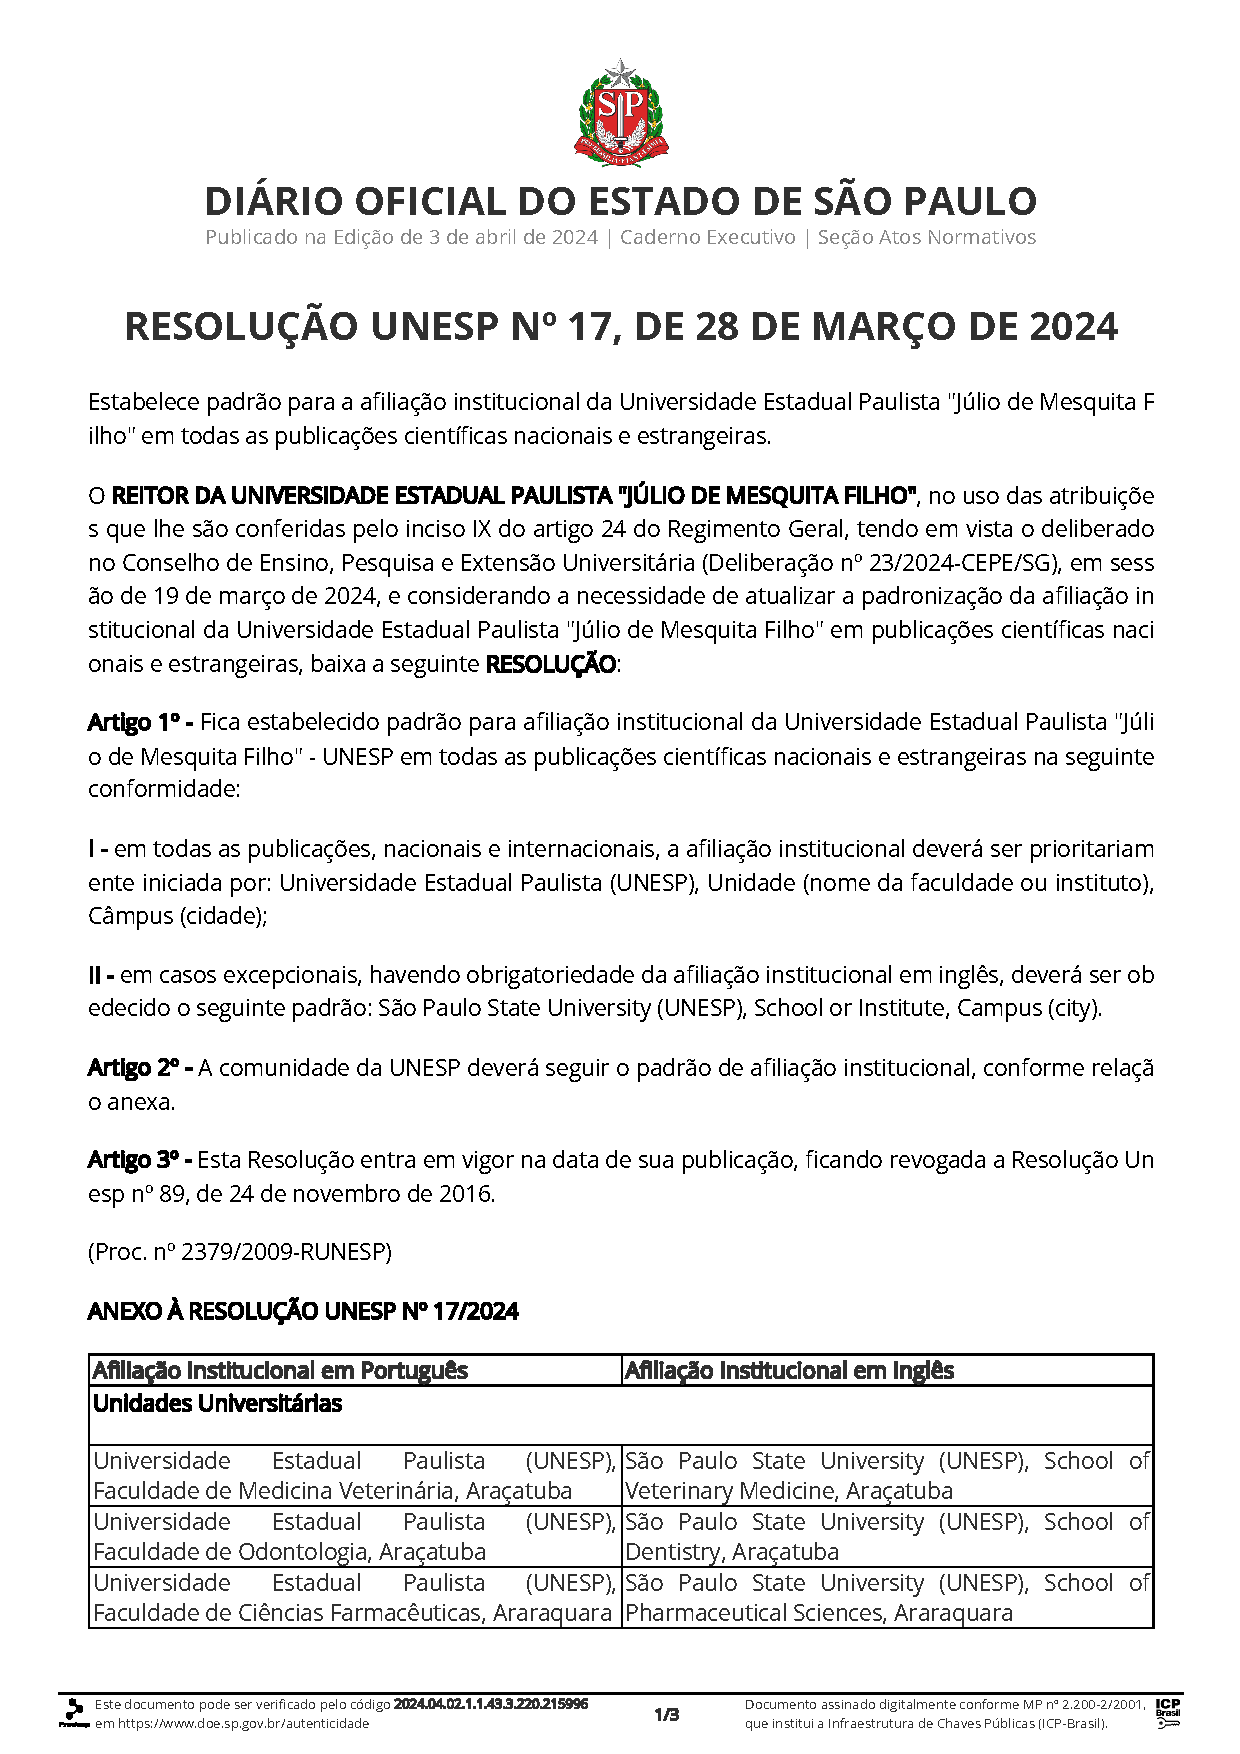
\includepdf[pages=-]{anexos/resolucao_unesp17-2024.pdf}
	
	
\end{anexosenv}
 	%
\chapter{Conclusão}

Denominado também de considerações finais, é a parte final do texto, onde são apresentadas conclusões correspondentes aos objetivos ou hipóteses. É um processo de síntese dos principais resultados, com comentários do autor e as contribuições trazidas pelo trabalho. 

%------------------------------------------------------------------------------------%
%                               P Ó S   T E X T U A L                                %
%                                                                                    %
% Fim do corpo do texto. A partir desse comando as indicações no sumário serão       %
% marcadas como 'pós textuais'.                                                      %
%------------------------------------------------------------------------------------%

  	
  	
\end{document}

